\documentclass{article} % For LaTeX2e
\usepackage{nips14submit_e,times}
\usepackage{hyperref}
\usepackage{url}
\usepackage{amssymb,amsmath,amsthm}
\usepackage{subfigure}
\usepackage{tikz}
\usepackage{graphicx}
\usepackage{enumitem}
\usepackage{multirow}
\usepackage{algorithm,algorithmic}
\usetikzlibrary{positioning,decorations.pathreplacing}


\def\gap{\hspace*{.2in}}
\newcommand{\sketchplan}[1]{[\emph{#1}]}

\NewDocumentCommand{\var}{O{s} m O{}}{%
  \ensuremath{#1_{#2}^{#3}}% add \vphantom{<bizarre sup>}
}
\usepackage{siunitx}

\newcommand\accnum[1]{\num[round-precision=3]{#1}}
\newcommand\pernum[1]{\num[round-precision=1]{#1}}
\newcommand\scnum[1]{\num[scientific-notation=true,round-precision=1]{#1}}
\newcommand\numt[1]{\num[round-precision=2,round-mode=figures,scientific-notation=true]{#1}}
\newcommand\numo[1]{\num[round-precision=1,round-mode=figures,scientific-notation=true]{#1}}
%\newcommand{\numo}[1]{
%\pgfmathparse{#1}\pgfmathprintnumberto[precision=1, assume math mode=true]{\pgfmathresult}{\roundednumber}\roundednumber
%}
%\newcommand{\numt}[1]{
%\pgfmathparse{#1}\pgfmathprintnumberto[precision=2, assume math mode=true]{\pgfmathresult}{\roundednumber}\roundednumber
%}

\newcommand{\figref}[1]{Figure~\ref{#1}}
\newcommand{\tabref}[1]{Table~\ref{#1}}
\newcommand{\secref}[1]{\S\ref{#1}}
\newcommand{\algref}[1]{Algorithm~\ref{#1}}
\newcommand{\pref}[1]{page~\pageref{#1}}
\newcommand{\vect}[1]{\boldsymbol{#1}} % vector
\newcommand{\mat}[1]{\boldsymbol{#1}}  % matrix
\newcommand{\defeq}{\ensuremath{\mathrel{\mathop:}=}}
\newcommand{\eqdef}{\ensuremath{=\mathrel{\mathop:}}}

\newcommand{\ipoint}[1]{\textit{\textbf{\color{darkgray}#1}}}
\newcommand{\todo}[1]{{\color{red}todo: #1}}
%\newcommand{\comment}[1]{{\color{blue}comment: #1}}
\renewcommand{\b}[1]{{#1}}
\newcommand{\grbf}[1]{\mbox{\boldmath${#1}$\unboldmath}} %\renewcommand{\grbf}[1] {\mathbf{#1}}
\newcommand{\ns}[1]{\ensuremath{\mathbb{#1}}}
\newcommand{\fs}[1]{\ensuremath{\mathcal{#1}}}
\newcommand{\idiv}{\ensuremath{\nabla\cdot}}
\newcommand{\igrad}{\ensuremath{\nabla}}
\newcommand{\ilap}{\rotatebox[origin=c]{180}{$\nabla$}}
\newcommand{\icurl}{\ensuremath{\nabla \times}}
\newcommand{\tr}{\ensuremath{\operatorname{tr}}}
\newcommand{\id}{\ensuremath{\operatorname{id}}}
\newcommand{\ts}{\textsuperscript}
\newcommand{\half}[1]{\frac{#1}{2}}
\renewcommand{\d}[1]{\mathop{}\!\mathrm{d}#1}
\newcommand{\dt}{\d{t}}
\newcommand{\dx}{\d{\vect{x}}}
\newcommand{\p} {\partial}
\newcommand{\op}[1]{\ensuremath{\mathcal{#1}}}
\newcommand{\di}[1]{\ensuremath{\mathbf{#1}}}


\DeclareMathOperator*{\argmin}{arg\,min}
\newcommand{\MA}[1]{{\mathcal #1}}
\DeclareMathOperator{\bigO}{\mathcal{O}}
\newcommand{\reals}{\mathbb{R}}
\newcommand{\codenm}[1]{{\tt  #1}}
\newcommand{\zapspace}{\topsep=0pt\partopsep=0pt\itemsep=0pt\parskip=0pt}

\newcommand{\msection}[1]{\vspace*{-5pt}\section{#1}\vspace{-4pt}}
\newcommand{\msubsection}[1]{\vspace*{-5pt}\subsection{#1}\vspace{-4pt}}
%\newcommand{\msection}[1]{\section{#1}}
%\newcommand{\msubsection}[1]{\subsection{#1}}


\definecolor{light-gray}{gray}{0.80}
%\renewcommand{\algorithmiccomment}[1]{#1}


\newcommand{\mcol}[2]{\multicolumn{#1}{r}{#2}}
\newcommand{\mrow}[2]{\multirow{#1}{*}{#2}}
\newcommand{\mrowrot}[2]{
\parbox[t]{2mm}{\multirow{#1}{*}{\rotatebox[origin=c]{90}{#2}}}
}


%\newcommand{\algcolor}[2]{\hspace*{-\fboxsep}\colorbox{#1}{\parbox{\linewidth}{#2}}}
\newcommand{\algcolor}[2]{\colorbox{#1}{\parbox{\linewidth}{#2}}}
\newcommand{\algemph}[1]{\algcolor{light-gray}{#1}}

\newcommand{\algcmt}[1]{\hfill {\footnotesize\ttfamily\textcolor{blue}{/* {#1} */}}}
%\newcommand{\algcmt}[1]{{\footnotesize\ttfamily\textcolor{blue}{\dotfill #1}}}
\newcommand{\algcc}[1]{\hfill {\footnotesize\ttfamily\textcolor{blue}{//{#1}}}}

\let\oldparagraph\paragraph
\renewcommand\paragraph{\subsubsection*}


\newcommand{\bfeval}[1]{
  \textcolor{black}{\textbf{\eval{#1}}}
}
\newcommand\aref{Algorithm \ref}
\newcommand\eref{Eq.~\ref}

\newcommand\fref{Fig.~\ref}
\newcommand\tref{Table~\ref}
\SetKwInOut{Parameter}{parameter}
\newcommand\cmt[1]{\tcp*[r]{\scriptsize \color{gray!80!black}#1}}
\newcommand{\red}[1]{{\color{red} #1}}
\newcommand{\blue}[1]{{\color{blue} #1}}
\newcommand{\bluem}[1]{{\bf\color{blue} #1}}
\newcommand\ha{ \rowcolor{orange!0}}
\newcommand\hb{ \rowcolor{orange!15}}
\newcommand\hc{ \rowcolor{orange!40}}
\newcommand\hd{ \rowcolor{orange!45}}
\newcommand\he{ \rowcolor{orange!60}}
\newcommand\hf{ \rowcolor{orange!75}}
\newcommand\hg{ \rowcolor{orange!90}}


\newcommand\eps{ \epsilon}
% notation simplification
\newcommand\MS{{\mathcal{M}}}
\def\x{{\bf x}}
\def\H{{\bf H}}
\def\g{{\bf g}}
\def\Hg{{\bf Hg}}
\def\0{{\bf 0}}
\def\s{{\bf s}}
\def\t{{\bf t}}
\def\p{{\bf p}}




\def\vv{{\bf v}}

\def\R{{\mathbb R}}

\def\AS{{\mathcal{A}}}


 % \newtheorem{remk}[theorem]{Remark}


\title{Convolutional Kernel Networks}

\author{
   Julien Mairal, Piotr Koniusz, Zaid Harchaoui, and Cordelia Schmid \\
   Inria\thanks{LEAR team, Inria Grenoble, Laboratoire Jean Kuntzmann, CNRS, Univ. Grenoble Alpes, France.} \\
   \texttt{firstname.lastname@inria.fr}
}

% The \author macro works with any number of authors. There are two commands
% used to separate the names and addresses of multiple authors: \And and \AND.
%
% Using \And between authors leaves it to \LaTeX{} to determine where to break
% the lines. Using \AND forces a linebreak at that point. So, if \LaTeX{}
% puts 3 of 4 authors names on the first line, and the last on the second
% line, try using \AND instead of \And before the third author name.

\newcommand{\fix}{\marginpar{FIX}}
\newcommand{\new}{\marginpar{NEW}}

\nipsfinalcopy % Uncomment for camera-ready version

\begin{document}


\maketitle

\begin{abstract}
   % \begin{figure}[h!]
%     \centering
%     \includegraphics[width=\linewidth,height=5cm]{fig/placeholder}
% \end{figure}

% While object recognition on 2D images is getting more and more mature, 3D understanding is eagerly in demand yet largely underexplored. In this paper, we study the 3D object detection problem from RGB-D data captured by depth sensors in both indoor and outdoor environments. Different from previous deep learning methods that work on 2D RGB-D images or 3D voxels, which often obscure natural 3D patterns and invariances of 3D data, we directly operate on raw point clouds by popping up RGB-D scans. Although recent works such as PointNet performs well for segmentation in small-scale point clouds, one key challenge is how to efficiently detect objects in large-scale scenes. Leveraging the wisdom of dimension reduction and mature 2D object detectors, we develop a Frustum PointNet framework that addresses the challenge. Evaluated on KITTI and SUN RGB-D 3D detection benchmarks, our method outperforms state of the arts by remarkable margins with high efficiency (running at 5 fps).


% While object recognition on 2D images is getting more and more mature, 3D understanding is eagerly in demand yet underexplored.
In this work, we study 3D object detection from RGB-D data in both indoor and outdoor scenes. While previous methods focus on images or 3D voxels, often obscuring natural 3D patterns and invariances of 3D data, we directly operate on raw point clouds by popping up RGB-D scans. However, a key challenge of this approach is how to efficiently localize objects in point clouds of large-scale scenes (region proposal). Instead of solely relying on 3D proposals, our method leverages both mature 2D object detectors and advanced 3D deep learning for object localization, achieving efficiency as well as high recall for even small objects. Benefited from learning directly in raw point clouds, our method is also able to precisely estimate 3D bounding boxes even under strong occlusion or with very sparse points. Evaluated on KITTI and SUN RGB-D 3D detection benchmarks, our method outperforms the state of the art by remarkable margins while having real-time capability.

\end{abstract}

\section{Introduction}
\section{Introduction}
\label{sec:intro}

Language modeling is among the important problems that require modeling long-term dependency, with successful applications such as unsupervised pretraining~\citep{dai2015semi,peters2018deep,radford2018improving,devlin2018bert}.
However, it has been a challenge to equip neural networks with the capability to model long-term dependency in sequential data.
Recurrent neural networks (RNNs), in particular Long Short-Term Memory (LSTM) networks~\citep{hochreiter1997long}, have been a standard solution to language modeling and obtained strong results on multiple benchmarks.
Despite the wide adaption, RNNs are difficult to optimize due to gradient vanishing and explosion~\citep{hochreiter2001gradient}, and the introduction of gating in LSTMs and the gradient clipping technique~\citep{graves2013generating} might not be sufficient to fully address this issue.
% ,pascanu2012understanding
Empirically, previous work has found that LSTM language models use 200 context words on average~\citep{khandelwal2018sharp}, indicating room for further improvement.

On the other hand, the direct connections between long-distance word pairs baked in attention mechanisms might ease optimization and enable the learning of long-term dependency~\citep{bahdanau2014neural,vaswani2017attention}.
Recently, \citet{al2018character} designed a set of auxiliary losses to train deep Transformer networks for character-level language modeling, which outperform LSTMs by a large margin.
Despite the success, the LM training in~\citet{al2018character} is performed on separated fixed-length segments of a few hundred characters, without any information flow across segments.
As a consequence of the fixed context length, the model cannot capture any longer-term dependency beyond the predefined context length.
In addition, the fixed-length segments are created by selecting a consecutive chunk of symbols without respecting the sentence or any other semantic boundary.
Hence, the model lacks necessary contextual information needed to well predict the first few symbols, leading to inefficient optimization and inferior performance.
We refer to this problem as \textit{context fragmentation}.

%However, the context length is fixed to hundreds of characters and thus it is not possible to model longer-term dependency. Moreover, it is not clear how the model performs on word-level language modeling data, as the granularity changes.

% Moreover, using auxiliary losses brings additional challenges such as properly tuning the mixture weights and the loss decay schedule.

To address the aforementioned limitations of fixed-length contexts, we propose a new architecture called Transformer-XL (meaning extra long).
We introduce the notion of recurrence into our deep self-attention network. In particular, instead of computing the hidden states from scratch for each new segment, we reuse the hidden states obtained in previous segments.
The reused hidden states serve as memory for the current segment, which builds up a recurrent connection between the segments.
As a result, modeling very long-term dependency becomes possible because information can be propagated through the recurrent connections.
Meanwhile, passing information from the previous segment can also resolve the problem of context fragmentation.
More importantly, we show the necessity of using relative positional encodings rather than absolute ones, in order to enable state reuse without causing temporal confusion.
Hence, as an additional technical contribution, we introduce a simple but more effective relative positional encoding formulation that generalizes to attention lengths longer than the one observed during training.

Transformer-XL obtained strong results on five datasets, varying from word-level to character-level language modeling.
Transformer-XL is also able to generate relatively coherent long text articles with \textit{thousands of} tokens (see Appendix \ref{sec:gen}), trained on only 100M tokens.
% Transformer-XL improves the previous state-of-the-art (SoTA) results from 1.06 to 0.99 in bpc on enwiki8, from 1.13 to 1.08 in bpc on text8, from 20.5 to 18.3 in perplexity on WikiText-103, and from 23.7 to 21.8 in perplexity on One Billion Word.
% Transformer-XL improves the previous state-of-the-art (SoTA) results to 0.99 in bpc on enwiki8, 1.08 in bpc on text8, 18.3 in perplexity on WikiText-103, and 21.8 in perplexity on One Billion Word.
% On small data, Transformer-XL also achieves a perplexity of 54.5 on Penn Treebank without finetuning, which is SoTA when comparable settings are considered.

Our main technical contributions include introducing the notion of recurrence in a purely self-attentive model and deriving a novel positional encoding scheme. These two techniques form a complete set of solutions, as any one of them alone does not address the issue of fixed-length contexts. Transformer-XL is the first self-attention model that achieves substantially better results than RNNs on both character-level and word-level language modeling.

% On WikiText-103, Transformer-XL improves the previous state-of-the-art (SoTA) results from 33 perplexity to 24, with a relative reduction of 27\%. On enwiki8 character-level language modeling, Transformer-XL achieves a SoTA bpc of 1.03, which outperforms \cite{al2018character} by 0.03 with 60+\% fewer parameters. Given a more common model size with 40+M parameters, Transformer-XL achieves a bpc of 1.06, compared to 1.11 by \cite{al2018character}. Transformer-XL also achieves perplexities of 54.5 on Penn Treebank and 29.4 on One Billion Word, which are SoTA when comparable settings are considered.

% Due to the ability of modeling long-range context, our best model uses attention lengths of 1,600 and 3,800 on WikiText-103 and enwiki8 respectively. We also devise a metric called \textit{Relative Effective Context Length} (RECL) that aims to fairly compare the ability of long-range dependency modeling.
% % perform a fair comparison of the gains brought by increasing the context lengths for different models.
% In this setting, Transformer-XL learns a RECL of 900 words on WikiText-103, while the numbers for recurrent networks and Transformer are only 500 and 128.

% We use two methods to quantitatively study the effective lengths of Transformer-XL and the baselines. Similar to \cite{khandelwal2018sharp}, we gradually increase the attention length at test time until no further noticeable improvement ($\sim$0.1\% relative gains) can be observed. Our best model in this settings use attention lengths of 1,600 and 3,800 on WikiText-103 and enwiki8 respectively.
% %In addition, since the effective context length of Transformer-XL can be longer than the attention length due to our recurrent formulation, we devise a metric called \textit{Relative Effective Context Length} (RECL) that aims to perform a fair comparison of the gains brought by increasing the context lengths for different models.
% In addition, we devise a metric called \textit{Relative Effective Context Length} (RECL) that aims to perform a fair comparison of the gains brought by increasing the context lengths for different models.
% In this setting, Transformer-XL learns a RECL of 900 words on WikiText-103, while the numbers for recurrent networks and Transformer are only 500 and 128.


\subsection{Related Work}\label{sec:related}
\paragraph{3D Object Detection from RGB-D Data} Researchers have approached the 3D detection problem by taking various ways to represent RGB-D data.

\emph{Front view image based methods:} ~\cite{chen2016monocular, mousavian20163d, xiang2015data} take monocular RGB images and shape priors or occlusion patterns to infer 3D bounding boxes. ~\cite{li2016vehicle, deng2017amodal} represent depth data as 2D maps and apply CNNs to localize objects in 2D image. In comparison we represent depth as a point cloud and use advanced 3D deep networks (PointNets) that can exploit 3D geometry more effectively.

\emph{Bird's eye view based methods:} MV3D~\cite{cvpr17chen} projects LiDAR point cloud to bird's eye view and trains a region proposal network (RPN~\cite{ren2015faster}) for 3D bounding box proposal. However, the method lags behind in detecting small objects, such as pedestrians and cyclists and cannot easily adapt to scenes with multiple objects in vertical direction.
%Our method shares the idea with~\cite{cvpr17chen} in reducing 3D search cost by 2D search first. What differentiates our method from \cite{cvpr17chen} is that, \hao{???} instead of projecting point cloud to images costing loss in 3D geometry, we directly apply PointNet to point clouds that correspond to the 2D regions. % Besides, our method and MV3D can potentially be combined in the bird's eye setting. 3D proposals from our frustum-based PointNet and MV3D can be combined and our 3D network can also be used for bounding box estimation for point cloud in the bird's eye 2D region.

\emph{3D based methods:} ~\cite{wang2015voting, song2014sliding} train 3D object classifiers by SVMs on hand-designed geometry features extracted from point cloud and then localize objects using sliding-window search. \cite{engelcke2017vote3deep} extends ~\cite{wang2015voting} by replacing SVM with 3D CNN on voxelized 3D grids. \cite{ren2016three} designs new geometric features for 3D object detection in a point cloud. \cite{song2016deep, li20163d} convert a point cloud of the entire scene into a volumetric grid and use 3D volumetric CNN for object proposal and classification. Computation cost for those method is usually quite high due to the expensive cost of 3D convolutions and large 3D search space.
%In comparison, we use 2D region proposals from RGB images to reduce the search space from the entire 3D scenes into 3D frustums. Since the points cloud in the frustums have largely varying depth ranges and can be very sparse, it's not applicable to apply CNN on bird's eye view or apply 3D CNN in grids. Our frustum-based PointNet, on the other hand, suits well for this type of data and is able to accurately estimate 3D bounding box with good efficiency.
Recently, \cite{lahoud20172d} proposes a 2D-driven 3D object detection method that is similar to ours in spirit. However, they use hand-crafted features (based on histogram of point coordinates) with simple fully connected networks to regress 3D box location and pose, which is sub-optimal in both speed and performance. In contrast, we propose a more flexible and effective solution with deep 3D feature learning (PointNets).
%In addition we also get 3D instance segmentation as intermediate outputs. Evaluated on SUN-RGBD we show our method is \emph{8.9\%} better than theirs in mAP and \emph{34x} faster at the same time.


% \begin{enumerate}
%     \item ZOOX~\cite{mousavian20163d} image based
%     \item Vote3Deep~\cite{engelcke2017vote3deep} 3d cnn. Recent LIDAR-based methods place 3D windows in 3D voxel grids to score the point cloud
%     \item Voting for Voting~\cite{wang2015voting} Recent LIDAR-based methods place 3D windows in 3D voxel grids to score the point cloud. apply SVM classifers on 3D grids encoded with geometry features
%     \item MV3D~\cite{cvpr17chen}
%     \item VeloFCN~\cite{li2016vehicle} apply convolutional networks to the front view point map in a dense box prediction scheme
%     \item 3DOP~\cite{chen20153d} image based. reconstructs depth from stereo images and uses an energy minimization approach to generate 3D box proposals, which are fed to an R-CNN [10] pipeline for object recognition
%     \item Mono3D~\cite{chen2016monocular} image based. shares the same pipeline with 3DOP, it generates 3D proposals from monocular images.
%     \item 3DFCN~\cite{li20163d} 3d cnn.
%     \item 3DVP~\cite{xiang2015data} introduces 3D voxel patterns and employ a set of ACF detectors to do 2D detection and 3D pose estimation
%     \item Are Cars just 3D Box?~\cite{zeeshan2014cars} fit model to image patch
%     \item ~\cite{zia2013detailed} fit model to image patch
% \end{enumerate}
% \begin{enumerate}
%     \item SlidingShapes~\cite{song2014sliding} apply SVM classifers on 3D grids encoded with geometry features
%     \item DeepSlidingShapes~\cite{song2015sun} 3d cnn.
%     \item 2D-driven~\cite{lahoud20172d}
%     \item ~\cite{deng2017amodal} rgb-d images
%     \item COG feature~\cite{ren2016three}
%     \item Align 3D model in RGB-D~\cite{gupta2015aligning}
% \end{enumerate}

\paragraph{Deep Learning on Point Clouds}
Most existing works convert point clouds to images or volumetric forms before feature learning. \cite{wu20153d, maturana2015voxnet, qi2016volumetric} voxelize point clouds into volumetric grids and generalize image CNNs to 3D CNNs. ~\cite{li2016fpnn, riegler2016octnet, wang2017cnn, engelcke2017vote3deep} design more efficient 3D CNN or neural network architectures that exploit sparsity in point cloud.
However, these CNN based methods still require quantitization of point clouds with certain voxel resolution.
Recently, a few works~\cite{qi2017pointnet,qi2017pointnetplusplus} propose a novel type of network architectures (PointNets) that directly consumes raw point clouds without converting them to other formats. While PointNets have been applied to single object classification and semantic segmentation, our work explores how to extend the architecture for the purpose of 3D object detection.

\section{Convolutional Multilayer Kernels}\label{sec:scattering}
\input{scattering.tex}

\section{Training Invariant Convolutional Kernel Networks}\label{sec:approx}
Generic schemes have been proposed for approximating a non-linear kernel with a
linear one, such as the Nystr\"om method and its
variants~\cite{bo2009,williams2001}, or random sampling techniques in the
Fourier domain for shift-invariant kernels~\cite{rahimi2007}.  In the context
of convolutional multilayer kernels, such an approximation is critical because
computing the full kernel matrix on a database of images is computationally
infeasible, even for a moderate number of images ($\approx 10\,000$) and
moderate number of layers. For this reason, Bo et al.~\cite{bo2011}
use the Nystr\"om method for their hierarchical kernel descriptors. 

In this section, we show that when the coordinate sets~$\Omega_k$ are 
two-dimensional regular grids, a natural approximation for the multilayer convolutional kernel consists of a sequence of
spatial convolutions with learned filters, pointwise non-linearities, and pooling
operations, as illustrated in Figure~\ref{subfig:convnet}. 
More precisely, our scheme approximates the kernel map of~$K$ defined
in~(\ref{eq:kernel}) at layer~$k$ by finite-dimensional spatial maps~$\xi_k: \Omega'_k \to \Real^{p_k}$, where~$\Omega'_k$ is a set of coordinates related to~$\Omega_k$,
and~$p_k$ is a positive integer controlling the quality of the approximation. 
Consider indeed two images represented at layer~$k$ by image
feature maps $\varphi_k$ and~$\varphi_k'$, respectively. Then,
\begin{itemize}[leftmargin=0.7cm]
   \item[{\bfseries (A)}] the corresponding maps~$\xi_k$ and~$\xi'_k$ are learned such that
      $K(\varphi_{\kmone},\varphi_{\kmone}') \approx \langle \xi_k, \xi_k' \rangle$, where~$\langle.,.\rangle$ is
      the Euclidean inner-product acting as if~$\xi_k$ and~$\xi_k'$ were vectors in~$\Real^{|\Omega_k'| p_k}$;
   \item[{\bfseries (B)}] the set~$\Omega'_k$ is linked to~$\Omega_k$ by the
      relation~$\Omega_k'\!=\!\Omega_k + \PP_k'$ where~$\PP_k'$ is a patch
      shape, and the quantities~$\varphi_k(\z_k)$ in~$\HH_k$ admit finite-dimensional 
      approximations~$\psi_k(\z_k)$ in~$\Real^{|\PP_k'|p_k}$; as
      illustrated in Figure~\ref{subfig:convnet}, $\psi_k(\z_k)$ is a patch
      from~$\xi_k$ centered at location~$\z_k$ with shape~$\PP_k'$;
   \item[{\bfseries (C)}] an activation map~$\zeta_{k}: \Omega_{\kmone} \mapsto \Real^{p_{k}}$ is computed from~$\xi_{\kmone}$ by 
      convolution with~$p_k$ filters followed by a non-linearity. The subsequent map~$\xi_k$ is obtained from~$\zeta_k$ by a
      pooling operation. 
\end{itemize}
We call this approximation scheme a convolutional kernel network
(CKN). In comparison to CNNs, our approach enjoys similar benefits such as efficient prediction at test
time, and involves the same set of hyper-parameters: number of layers, numbers
of filters~$p_k$ at layer~$k$, shape~$\PP_k'$ of the filters, sizes of the feature maps.
The other parameters~$\beta_k, \sigma_k$ can be automatically chosen, as
discussed later. Training a CKN can be argued to be as simple as
training a CNN in an unsupervised manner~\cite{ranzato2007} since we will show that
the main difference is in the cost function that is optimized.


\subsection{Fast Approximation of the Gaussian Kernel}\label{subsec:approx_gaussian}
A key component of our formulation is the Gaussian kernel. We start by
approximating it by a linear operation with learned filters followed by a
pointwise non-linearity.  Our starting point is the next lemma, which can be
obtained after a simple calculation.
\begin{lemma}[\bfseries Linear expansion of the Gaussian Kernel]
   For all~$\x$ and~$\x'$ in~$\Real^m$, and~$\sigma > 0$, 
   \begin{equation}
      e^{-\frac{1}{2\sigma^2}\|\x-\x'\|_2^2} = \left(\frac{2}{\pi \sigma^2}\right)^{\frac{m}{2}} \int_{\w \in \Real^m} e^{-\frac{1}{\sigma^2}\|\x-\w\|_2^2}e^{-\frac{1}{\sigma^2}\|\x'-\w\|_2^2} d\w.\label{eq:rbf}
   \end{equation}
\end{lemma}
The lemma gives us a mapping of any~$\x$ in~$\Real^m$ to the function $\w
\mapsto \sqrt{C} e^{-(1/\sigma^2)\|\x-\w\|_2^2}$ in $L^2(\Real^m)$, where the
kernel is linear, and $C$ is the constant in front of the integral. 
To obtain a finite-dimensional representation, we need
to approximate the integral with a weighted finite sum, which is a
classical problem arising in statistics~(see \cite{wahba} and chapter 8 of~\cite{bottou2007}). 
Then, we consider two different~cases.
\vspace*{-0.2cm}
\paragraph{Small dimension, $m \leq 2$.}
When the data lives in a compact set of~$\Real^m$, the
integral in~(\ref{eq:rbf}) can be approximated by uniform sampling over a large
enough set. We choose such a strategy for two types of kernels from Eq.~(\ref{eq:kernel}):
(i) the spatial kernels~$e^{-\left(\frac{1}{2\beta^2}\right)\left\|\z-\z'\right\|_2^2}$;
(ii) the terms $e^{-\left(\frac{1}{2\sigma^2}\right)\left\|\tildephi(\z)-\tildephi'(\z')\right\|_\HH^2}$ when
$\varphi$ is the ``gradient map'' presented in Section~\ref{sec:scattering}. In
the latter case, $\HH = \Real^2$ and $\tildephi(\z)$ is the gradient orientation.
We typically sample a few orientations as explained in Section~\ref{sec:exp}.

\vs
\paragraph{Higher dimensions.}
To prevent the curse of dimensionality, we learn to
approximate the kernel on training data, which is intrinsically
low-dimensional. We optimize importance weights~$\etab=[\eta_l]_{l=1}^p$
in~$\Real_+^p$ and sampling points $\W = [\w_l]_{l=1}^p$ in~$\Real^{m \times
p}$ on~$n$ training pairs~$(\x_i,\y_i)_{i=1,\ldots,n}$ in~$\Real^m \times
\Real^m$:
\begin{equation}
   \min_{\etab \in \Real_+^p, \W \in \Real^{m \times p}} \bigg[ \frac{1}{n} \sum_{i=1}^n \Big(e^{-\frac{1}{2\sigma^2}\|\x_i-\y_i\|_2^2} - \sum_{l=1}^p \eta_l e^{-\frac{1}{\sigma^2}\|\x_i-\w_l\|_2^2} e^{-\frac{1}{\sigma^2}\|\y_i-\w_l\|_2^2}\Big)^2   \bigg]. \label{eq:opt}
\end{equation}
Interestingly, we may already draw some links with neural networks. When
applied to unit-norm vectors $\x_i$ and~$\y_i$,
problem~(\ref{eq:opt}) produces sampling points~$\w_l$ whose norm is close to
one. After learning, a new unit-norm point~$\x$ in~$\Real^m$ is mapped to the
vector $[\sqrt{\eta_l} e^{-({1}/{\sigma^2})\|\x-\w_l\|_2^2}]_{l=1}^p$ in~$\Real^p$,
which may be written as $[f(\w_l^\top \x)]_{l=1}^p$, assuming that the norm of~$\w_l$ is always one, where $f$ is the
function $u \mapsto e^{(2/\sigma^2)(u -1)}$ for
$u=\w_l^\top\x$ in~$[-1, 1]$.  
Therefore, the finite-dimensional representation of~$\x$ only involves a linear
operation followed by a non-linearity, as in typical neural networks.  In
Figure~\ref{fig:relu}, we show that the shape of~$f$ resembles the ``rectified
linear unit'' function~\cite{wan2013}.
\pgfsetlayers{main}
\begin{figure}[hbtp]
   \centering
   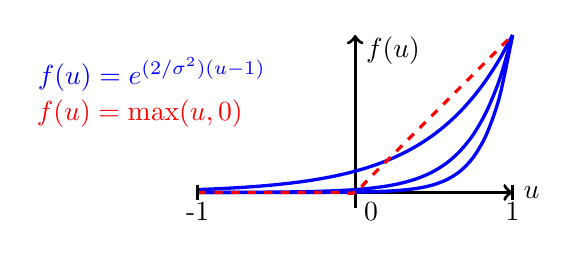
\begin{tikzpicture}[scale=2]
      \draw[->,very thick,black] (-1,0) -- (1,0) node[right] {$u$};
      \draw[->,very thick,black] (0,-0.1) -- (0,1) node[right,yshift=-2mm] {$f(u)$};
      \draw[scale=1,domain=-1:1,smooth,variable=\x,very thick,blue] plot ({\x},{exp(2*(\x-1))});
      \draw[scale=1,domain=-1:1,smooth,variable=\x,very thick,blue] plot ({\x},{exp(4*(\x-1))}) node[left,xshift=-3cm,yshift=-0.5cm] {$f(u)=e^{(2/\sigma^2)(u-1)}$};
      \draw[scale=1,domain=-1:1,smooth,variable=\x,very thick,blue] plot ({\x},{exp(6*(\x-1))});
      \draw[scale=1,domain=-1:1,smooth,variable=\x,very thick,dashed,red] plot ({\x},{max(\x,0)}) node[left,xshift=-3.29cm,yshift=-1cm] {$f(u)=\max(u,0)$};
      \draw (0,0) node[anchor=north,xshift=2mm] {0};
      \draw (1,0) node[anchor=north] {1};
      \draw (-1,0) node[anchor=north] {-1};
      \draw[very thick] (-1,0.05) -- (-1,-0.05);
      \draw[very thick] (1,0.05) -- (1,-0.05);
   \end{tikzpicture}
   \vspace*{-0.3cm}
   \caption{In dotted red, we plot the ``rectified linear unit'' function $u \mapsto \max(u,0)$. In blue, we plot non-linear functions of our network for typical values of~$\sigma$ that we use in our experiments.}\label{fig:relu}
\end{figure}

\vspace*{-0.3cm}
\subsection{Approximating the Multilayer Convolutional Kernel}

We have now all the tools in hand to build our convolutional kernel network.
We start by making assumptions on the input data, and then present the learning scheme and its approximation principles.

\vs
\paragraph{The zeroth layer.} We assume that the input data is a
finite-dimensional map $\xi_0: \Omega_0' \to \Real^{p_0}$, and that $\varphi_0:
\Omega_0 \to \HH_0$ ``extracts'' patches from~$\xi_0$. Formally, there
exists a patch shape~$\PP_0'$ such that $\Omega_0' = \Omega_0 + \PP_0'$, $\HH_0
= \Real^{p_0|\PP_0'|}$, and for all $\z_0$ in~$\Omega_0$, $\varphi_0(\z_0)$ is
a patch of $\xi_0$ centered at~$\z_0$. 
Then, property {\bfseries (B)} described at the beginning of
Section~\ref{sec:approx} is satisfied for $k\!=\!0$ by choosing
$\psi_0\!=\!\varphi_0$. The examples of input feature maps given earlier
satisfy this finite-dimensional assumption: for the gradient map, $\xi_0$ is
the gradient of the image along each direction, with $p_0=2$, $\PP_0'=\{ 0\}$
is
a $1 \!\times \!1$ patch, $\Omega_0\!=\!\Omega_0'$, and $\varphi_0\!=\!\xi_0$;
for the patch map, $\xi_0$ is the input image, say with $p_0\!=\!3$ for RGB data.


\vs
\paragraph{The convolutional kernel network.}
The zeroth layer being characterized, we present in Algorithms~\ref{alg:ckn}
and~\ref{alg:ckn2} the subsequent layers and how to learn their parameters 
in a feedforward manner. It is interesting to note that the input parameters of
the algorithm are exactly the same as a CNN---that is, number of layers and filters,
sizes of the patches and feature maps (obtained here via the subsampling factor).
Ultimately, CNNs and CKNs only differ in the cost function that is
optimized for learning the filters and in the choice of non-linearities.  As we
show next, there exists a link between the parameters of a CKN and those of
a convolutional multilayer kernel.

\begin{algorithm}
   \caption{Convolutional kernel network - learning the parameters of the $k$-th layer.}\label{alg:ckn}
   \begin{algorithmic}[1]
      \INPUT $\xi^1_{\kmone}, \xi^2_{\kmone},\ldots: \Omega'_{\kmone} \to \Real^{p_{\kmone}}$ (sequence of $(\kmone)$-th maps obtained from training images); $\PP_{\kmone}'$ (patch shape); $p_k$ (number of filters); $n$ (number of training pairs);
      \STATE extract at random $n$ pairs $(\x_i,\y_i)$ of patches with shape $\PP_{\kmone}'$ from the maps~$\xi_{\kmone}^1,\xi_{\kmone}^2,\ldots$;
      \STATE if not provided by the user, set $\sigma_k$ to the~$0.1$ quantile of the data~($\|\x_i-\y_i\|_2)_{i=1}^n$;
      \STATE {\bfseries unsupervised learning:} optimize~(\ref{eq:opt}) to obtain the filters~$\W_k$ in~$\Real^{|\PP_{\kmone}'|p_{\kmone} \times p_k}$ and $\etab_k$ in~$\Real^{p_k}$;
      \OUTPUT $\W_k$, $\etab_k$, and $\sigma_k$ (smoothing parameter);
   \end{algorithmic}
\end{algorithm}
\begin{algorithm}
   \caption{Convolutional kernel network - computing the $k$-th map form the~$(\kmone)$-th one.}\label{alg:ckn2}
   \begin{algorithmic}[1]
      \INPUT $\xi_{\kmone}: \Omega'_{\kmone} \!\to\! \Real^{p_{\kmone}}$ (input map); $\PP_{\kmone}'$ (patch shape); $\gamma_k \!\geq \!1$ (subsampling factor); $p_k$ (number of filters); $\sigma_k$ (smoothing parameter); $\W_k=[\w_{kl}]_{l=1}^{p_k}$ and~$\etab_k=[\eta_{kl}]_{l=1}^{p_k}$ (layer parameters);
      \STATE {\bfseries convolution and non-linearity:} define the activation map $\zeta_k: \Omega_{\kmone} \to \Real^{p_k}$ as
      \begin{equation}
         \vsb
         \zeta_k: \z \mapsto \|\psi_{\kmone}(\z)\|_2 \left[\sqrt{\eta_{kl}} e^{-\frac{1}{\sigma_k^2}\left\|\tildepsi_{\kmone}(\z)-\w_{kl}\right\|_2^2}\right]_{l=1}^{p_k}, \label{eq:zeta}
      \end{equation}
      where~$\psi_{\kmone}(\z)$ is a vector representing a patch from~$\xi_{\kmone}$ centered at~$\z$ with shape $\PP_{\kmone}'$, and the vector $\tildepsi_{\kmone}(\z)$ is an $\ell_2$-normalized version of~$\psi_{\kmone}(\z)$. This operation can be interpreted as a spatial convolution of the map~$\xi_{\kmone}$ with the filters~$\w_{kl}$ followed by pointwise non-linearities;
      \STATE set~$\beta_k$ to be~$\gamma_k$ times the spacing between two pixels in~$\Omega_{\kmone}$;
      \STATE {\bfseries feature pooling:}
      $\Omega'_k$ is obtained by subsampling~$\Omega_{\kmone}$ by a factor~$\gamma_k$ and we define a    
      new map $\xi_{k}: \Omega'_k \to \Real^{p_k}$ obtained from~$\zeta_k$ by linear pooling with Gaussian weights:
      \begin{equation}
         \vsb
         \xi_k: \z \mapsto \sqrt{{2}/\pi}\sum_{\u \in \Omega_{\kmone}}  e^{-\frac{1}{\beta_k^2}\left\|\u - \z\right\|_2^2} \zeta_k(\u). \label{eq:xi}
      \end{equation}
      \OUTPUT $\xi_{k} : \Omega'_k \to \Real^{p_k}$ (new map);
   \end{algorithmic}
\end{algorithm}

\paragraph{Approximation principles.}
\vspace*{-0.75cm}
We proceed recursively to show that the kernel approximation
property~{\bfseries (A)}
is satisfied; we assume that~{\bfseries (B)}
holds at layer~$\kmone$, and then, we show that {\bfseries (A)} and
{\bfseries (B)} also hold at layer~$k$.  This is sufficient for our 
purpose since we have previously assumed~{\bfseries (B)} for the zeroth layer.  
Given two images feature maps~$\varphi_{\kmone}$ and~$\varphi_{\kmone}'$, we 
start by approximating $K(\varphi_{\kmone},\varphi_{\kmone}')$ by replacing
$\varphi_{\kmone}(\z)$ and $\varphi_{\kmone}'(\z')$ by their finite-dimensional
approximations provided by~{\bfseries (B)}: 
\begin{equation}
   K(\varphi_{\kmone},\varphi_{\kmone}') \approx 
   \sum_{\z,\z' \in \Omega_{\kmone}} \normE{\psi_{\kmone}(\z)}  \normE{\psi_{\kmone}'(\z')} e^{-\frac{1}{2\beta_{k}^2}\normE{\z-\z'}^2} e^{-\frac{1}{2\sigma_k^2} \normE{\tildepsi_{\kmone}(\z)-\tildepsi_{\kmone}'(\z')}^2}.
\end{equation}
Then, we use the finite-dimensional approximation of the Gaussian kernel
involving~$\sigma_k$ and
\begin{equation}
         \vsb
   K(\varphi_{\kmone},\varphi_{\kmone}') \approx 
   \sum_{\z, \z' \in \Omega_{\kmone}} \zeta_k(\z)^\top \zeta_k'(\z') e^{-\frac{1}{2\beta_k^2}\normE{\z-\z'}^2},
\end{equation}
where~$\zeta_k$ is defined in~(\ref{eq:zeta}) and $\zeta_k'$ is defined
similarly by replacing~$\tildepsi$ by~$\tildepsi'$.  Finally, we approximate
the remaining Gaussian kernel by uniform sampling on $\Omega_{k}'$,
following Section~\ref{subsec:approx_gaussian}.
After exchanging sums and grouping appropriate terms together, we obtain the new approximation 
\begin{equation}
   K(\varphi_{\kmone},\varphi_{\kmone}') \approx \frac{2}{\pi} \sum_{\u \in \Omega_{k}'} \bigg( \sum_{\z \in \Omega_{\kmone}} e^{-\frac{1}{\beta_k^2}\normE{\z-\u}^2}\zeta_k(\z) \bigg)^\top \bigg( \sum_{\z' \in \Omega_{\kmone}}  e^{-\frac{1}{\beta_k^2}\normE{\z'-\u}^2} \zeta_k'(\z')  \bigg), \label{eq:approx}
\end{equation}
where the constant~$2/\pi$ comes from the multiplication of the constant
$2/(\pi\beta_k^2)$ from~(\ref{eq:rbf}) and the weight $\beta_k^2$ of uniform sampling
orresponding to the square of the distance between two pixels
of~$\Omega_k'$.\footnote{The choice of~$\beta_k$ in Algorithm~\ref{alg:ckn2} is
driven by signal processing principles. The feature pooling step can indeed be
interpreted as a downsampling operation that reduces the resolution of the map
from~$\Omega_{\kmone}$ to~$\Omega_k$ by using a Gaussian anti-aliasing filter,
whose role is to reduce frequencies
above the Nyquist limit.} As a result, the right-hand side is exactly $\langle
\xi_{k}, \xi_k' \rangle$, where~$\xi_k$ is defined in~(\ref{eq:xi}), giving us
property~{\bfseries (A)}. It remains to show that property~{\bfseries (B)} also
holds, specifically that the quantity~(\ref{eq:kernelpatch}) can be
approximated by the Euclidean inner-product~$\langle\psi_{k}(\z_k),
\psi'_k(\z_k')\rangle$ with the patches~$\psi_k(\z_k)$ and~$\psi'_k(\z_k')$ of shape~$\PP_k'$; we assume for that purpose that~$\PP_k'$ is a
subsampled version of the patch shape~$\PP_k$ by a factor~$\gamma_k$.

We remark that the kernel~(\ref{eq:kernelpatch}) is the same
as~(\ref{eq:kernel}) applied to layer~$\kmone$ by replacing~$\Omega_{\kmone}$
by~$\{\z_k\}+\PP_k$. By doing the same substitution in~(\ref{eq:approx}), we
immediately obtain an approximation of~(\ref{eq:kernelpatch}). Then, all
Gaussian terms are negligible for all~$\u$ and~$\z$ that are far from each
other---say when $\|\u-\z\|_2 \geq 2\beta_k$. Thus, we may replace the
sums~$\sum_{\u \in \Omega_k'}\sum_{\z,\z' \in \{\z_k\}+\PP_k}$ by~$\sum_{\u \in \{\z_k\}+\PP_k'}\sum_{\z,\z' \in \Omega_{\kmone}}$,
which has the same set of ``non-negligible'' terms. This yields exactly the
approximation $\langle\psi_{k}(\z_k), \psi'_k(\z_k')\rangle$.

\vs
\paragraph{Optimization.} 
Regarding problem~(\ref{eq:opt}), stochastic gradient descent
(SGD) may be used since a potentially infinite amount of training
data is available. However, we have preferred to use
L-BFGS-B~\cite{byrd1995} on $300\,000$ pairs of randomly selected training data
points, and initialize~$\W$ with the K-means algorithm. L-BFGS-B
is a parameter-free state-of-the-art batch method, which is not as
fast as SGD but much easier to use. We always run the L-BFGS-B algorithm for~$4\,000$ iterations, which seems to ensure
convergence to a stationary point. Our goal is to demonstrate the preliminary
performance of a new type of convolutional network, and we leave as future work
any speed improvement. 
\vsb


\section{Experiments}\label{sec:exp}
\begin{table*}[t!]
\centering
\small
\begin{tabular}{@{}p{0.09\linewidth}|p{0.04\linewidth}|p{0.025\linewidth}p{0.025\linewidth}p{0.025\linewidth}p{0.025\linewidth}p{0.03\linewidth}p{0.025\linewidth}p{0.025\linewidth}p{0.025\linewidth}p{0.03\linewidth}p{0.03\linewidth}p{0.025\linewidth}p{0.03\linewidth}p{0.03\linewidth}p{0.03\linewidth}p{0.03\linewidth}p{0.03\linewidth}}
\hline
category & mean & plane & bag & cap & car & chair & ear-phone & guitar & knife & lamp & laptop & motor-bike & mug & pistol & rocket & skate-board & table \\ \hline
Wu14 \cite{wu2014interactive} & - & 63.20 & - & - & - & 73.47 & - & - & - & 74.42 & - & - & - & - & - & - & 74.76 \\
Yi16 \cite{Yi16} & 81.43 & 80.96 & 78.37 & 77.68 & \textbf{75.67} & 87.64 & 61.89 & 91.79 & 85.36 & 80.59 & 95.58 & \textbf{70.59} & 91.85 & \textbf{85.94} & 53.13 & 69.81 & 75.33 \\
ACNN \cite{boscaini2016learning} & 79.63 & 76.35 & 72.89 & 70.80 & 72.72 & 86.12 & 71.14 & 87.84 & 81.98 & 77.43 & 95.49 & 45.68 & 89.49 & 77.41 & 49.23 & 82.05 & 76.71 \\
Voxel CNN & 79.37 & 75.14 & 72.80 & 73.28 & 70.00 & 87.17 & 63.50 & 88.35 & 79.58 & 74.43 & 93.92 & 58.67 & 91.79 & 76.41 & 51.16 & 65.25 & 77.08   \\ \hline
Ours1 & 83.48 & 80.61 & 81.62 & 76.92 & 73.86 & 88.65 & 74.48 & 89.03 & 85.34 & 83.47 & 95.53 & 62.74 & 92.01 & 80.88 & \textbf{62.10} & 82.23 & 81.36 \\
Ours2 & \textbf{84.74} & \textbf{81.55} & \textbf{81.74} & \textbf{81.94} & 75.16 & \textbf{90.24} & \textbf{74.88} & \textbf{92.97} & \textbf{86.10} & \textbf{84.65} & \textbf{95.61} & 66.66 & \textbf{92.73} & 81.61 & 60.61 & \textbf{82.86} & \textbf{82.13} \\ \hline
\end{tabular}
\caption{IoU for part segmentation on 16 categories. To compute mean IoU, per category IoU is weighted by the corresponding shape number and then averaged. Ours1 represents a variation of our framework without SpecTN and Ours2 corresponds to our full pipeline with SpecTN. On average, our approach outperforms all the baseline including both traditional machine learning and deep learning based methods by a large margin. We also achieves the highest IoU on most of the categories.}
\label{tab:percatseg}
\end{table*}
\label{sec:exp}
Our proposed SyncSpecCNN takes one graph vertex function as input and predicts another as output. As a generic framework, the prediction is not limited to a specific type of graph vertex function and can be tailored towards different goals. To evaluate the effectiveness of our framework, we divide our experiments into five parts. First, we evaluate on a benchmark of 3D shape segmentation~\cite{shapenet2015,Yi16}. Second, we evaluate on keypoint prediction task using a new large scale keypoint annotation dataset. Third, we leverage SyncSpecCNN to learn vertex normal functions and visualize the prediction results qualitatively. Fourth, we perform control experiments to compare different design choices of the framework and analyze the stability of our system under input sampling density variations. Last, we show qualitative results and analyze error patterns.

\subsection{Dataset}
For 3D shape segmentation task, we use a large scale shape part annotation dataset introduced by \cite{Yi16}, which augments a subset of ShapeNet models with semantic part annotations. The dataset contains 16 categories of man-made shapes, with 2 to 6 parts per category. In total there are 16,881 models with expert verified part annotations. In addition, we use the official train/test split provided along with ShapeNet models.

For the keypoint prediction task, we build a new large scale keypoint annotation dataset, containing 1,337 chair models with 10 keypoints per shape, in contrast to traditional small scale dataset \cite{kim2013learning} which has at most 100 shapes annotated per category. These keypoints are all manually annotated by experts with consistency across different shapes. %The goal of this dataset is to allow people evaluating data-driven keypoint prediction algorithms, in contrast to traditional small scale dataset \cite{kim2013learning} which has at most 100 shapes annotated per category.

\subsection{Shape Part Segmentation} 

\myparaly{Per-category shape part segmentation}
We first conduct part segmentation assuming the category label of each shape is known, as the setting in \cite{Yi16}. The task is to predict a part label for each sample point on shapes. We compare our framework with traditional learning-based techniques \cite{wu2014interactive,Yi16} leveraging on local geometric features and shape alignment cues, as well as recent deep learning based approaches \cite{boscaini2016learning} which also fall into the family of spectral CNNs. In addition we design an additional baseline using a 3D volumetric CNN architecture, denoted as Voxel CNN, which generalizes VoxNet~\cite{maturana2015voxnet} for segmentation tasks. The network has 10 convolutional layers without down-sampling and keeps a receptive field of 19 with spatial resolution of 32. We compute per-point features in the preprocessing step as is in \cite{Yi16} and use the same set of input for all baselines except Voxel CNN. The set of input shapes are pre-aligned using a hierarchical joint alignment algorithm described in \cite{shapenet2015}. Point intersection over union (IoU) is used as evaluation metric, averaged across all part classes. Cross-entropy loss is minimized during training. 

We evaluate our framework in two settings, with or without SpecTN, and compare the results in Table~\ref{tab:percatseg}. % In practice, we find that the gain from dilation becomes marginal when SpecTN is used, even though dilation alone helps significantly. While leaving out SpecTN, 
% We used our dilated parametrization with a dilation parameter $\gamma=128$ for convolution.
%We set a dilation parameter $\gamma=128$ for convolution.

Note that on most categories our approach achieves the best performance and on average outperforms state of the art by a large margin. In comparison to \cite{boscaini2016learning},  the state of the art in the family of spectral CNNs, our approach introduces spectral dilated kernel parametrization, which increases the effectiveness of spectral CNN framework.  Moreover, the performance gain from SpecTN shows that synchronizing spectral domains would greatly increase the generalizibility across shapes of different topology and geometry. 

\iffalse
\begin{table*}[t!]
\centering
\small
\begin{tabular}{@{}p{0.04\linewidth}|p{0.05\linewidth}p{0.07\linewidth}|p{0.025\linewidth}p{0.022\linewidth}p{0.022\linewidth}p{0.022\linewidth}p{0.025\linewidth}p{0.025\linewidth}p{0.025\linewidth}p{0.025\linewidth}p{0.025\linewidth}p{0.025\linewidth}p{0.025\linewidth}p{0.025\linewidth}p{0.025\linewidth}p{0.025\linewidth}p{0.025\linewidth}p{0.025\linewidth}}
\hline
& mean partial & mean complete & plane & bag & cap & car & chair & ear-phone & guitar & knife & lamp & laptop & motor-bike & mug & pistol & rocket & skate-board & table \\ \hline
ACNN & 69.21 & 79.63 & 62.73 & 63.26 & 58.90 & 38.25 & 70.59 & \textbf{68.68} & \textbf{88.08} & 74.58 & 61.49 & 87.03 & 31.90 & 79.92 & 62.98 & 35.70 & 68.41 & 76.07 \\ \hline
Ours1 & 76.19 & 83.48 & 71.01 & 77.61 & 64.78 & 56.05 & 78.97 & 68.50 & 84.63 & 82.01 & 73.02 & 91.40 & 40.71 & 87.34 & 72.60 & \textbf{42.53} & 80.61 & 79.55 \\
Ours2 & \textbf{78.02} & \textbf{84.74} & \textbf{74.55} & \textbf{82.58} & \textbf{65.36} & \textbf{58.12} & \textbf{80.41} & 65.55 & 84.75 & \textbf{82.53} & \textbf{77.39} & \textbf{93.15} & \textbf{43.12} & \textbf{90.24} & \textbf{74.71} & 42.17 & \textbf{83.22} & \textbf{80.51} \\ \hline
\end{tabular}
\caption{IoU for part segmentation on incomplete shapes. Note that for comparison, we not only report mean IoU for partial shape part segmentation under "mean partial", but also list mean IoU for complete shape part segmentation under "mean complete". Ours1 represents a variation of our framework without SpecTN and Ours2 corresponds to our full pipeline with SpecTN. On avearge we beat ACNN, the baseline approach, by a large margin and we outperforms ACNN on most shape categories. Moreover, our approach is more robust to data incompleteness since its performance drop is lower in comparison with complete shape segmentation.}
\label{tab:partialseg}
\end{table*}
\fi

\mypara{Cross-category shape part segmentation}
Next we evaluate our approach on the part segmentation task in a cross-category setting. In this task, shape category label is not known during the test phase and for each point the network needs to select one of the part label from all possible part labels in all categories. Cross-category setting introduces larger geometric and topological variance among shapes, thus could help examining the spectral CNN's ability of recognizing objects. At the same time the impact of spectral domain misalignment becomes stronger, providing a better testbed for validating the effectiveness of SpecTN. % Essentially the network needs to have the ability to differentiate shape categories in order to do this task well. 
% Since previous supervised shape segmentation approaches mostly focus on the setting with know shape category labels, 
Since this experiment is proposed to verify design choices of spectral CNN, we mainly compare with \cite{boscaini2016learning}. We mix the 16 categories of shapes in \cite{Yi16} and train a single network for all categories. After predicting point segmentation labels, one can classify shapes through a point-wise majority voting scheme. Point IoU and classification accuracy (Acc) are chosen as the evalution metric for part segmentation and object categorization, respectively. The results are shown in the $2$nd and $3$rd column of Table~\ref{tab:partialseg}.

Our approach outperforms the baseline ACNN by a large margin on both segmentation and classification. Note that ACNN~\cite{boscaini2016learning} does not explicitly conduct multi-scale analysis and is designed for near-isometric 3D shapes with similar spectral domains, thus generalizes less well across a diverse set of shapes. Our framework, in contrast, could effectively capture multi-scale context information, a feature that is highly important for both segmentation and classification. The spectral domain synchronization ability of SpecTN  further improves our generalizability, leading to an extra performance gain as is shown in Table~\ref{tab:partialseg}.

\iffalse
\begin{table}[h!]
\centering
\begin{tabular}{@{}ccc}
\toprule
               & IoU & Classification Acc\\ \midrule
ACNN \cite{boscaini2016learning} & 69.22 & 93.99 \\
Ours without SpecTN  & 79.65 & 99.59 \\
Ours with SpecTN  & \textbf{81.97} & \textbf{99.71} \\ \bottomrule
\end{tabular}
\caption{IoU for cross category part segmentation along with an induced classification accuracy. Even without SpecTN, our approach outperforms the baseline method on both segmentation IoU and classification accuracy, due to its ability of aggregating mult-scale information. Introducing SpecTN further improves the generalizability, resulting in an extra performance gain. }
\label{tab:crosscatseg}
\end{table}
\fi

\mypara{Partial data part segmentation}
To evaluate the robustness of our approach to incomplete data, we conduct part segmentation on simulated scans of 3D shapes from a single viewpoint. To be specific, we generate $N=6$ simulated scans for each 3D shape in the part annotation dataset \cite{Yi16} from random viewpoints, and then use these partial point cloud with part annotations for train and test. All the partial point clouds are normalized to fit into a unit cube. Following the train/test split provided by \cite{shapenet2015}, we train our network to segment shape parts for each category. Again we compare our method with ACNN~\cite{boscaini2016learning}. IoU is used as evaluation metric and the results are shown in the $4$th and $5$th column of Table~\ref{tab:partialseg}.

Our approach outperforms the baseline on partial data part segmentation by a large margin. In particular, from complete shape to partial shape setting, the performance drop of our approach is less significantly than the baseline, reflected by the gap of mean IoU between the complete data setting and the partial setting. It verifies that our method is more robust to data incompleteness. We surmise that the performance of ACNN is heavily influenced by noisy and sensitive principal curvature estimation on partial scans since this step plays a crucial rule in determining its local frames; whereas our approach makes less assumption about quality of the underlying shape.

\begin{table}[t!]
\centering
\small
\begin{tabular}{@{}c|cc|cc}
\hline
& cross cat IoU & Acc & partial & complete\\ \hline
ACNN & 69.22 & 93.99 & 69.21 & 79.63 \\ \hline
Ours1 & 79.65 & 99.59 & 76.19 & 83.48 \\
Ours2 & \textbf{81.97} & \textbf{99.71} & \textbf{78.02} & \textbf{84.74} \\ \hline
\end{tabular}
\caption{The $2$nd and $3$rd column of the table reports IoU for cross category part segmentation along with an induced classification accuracy. $4$th and $5$th column of the table reports IoU for part segmentation on partial shapes and complete shapes correspondingly. Our1 and Our2 corresponds to our framework without and with SpecTN respectively. In all experiments we beat the baseline by a large margin.}
\label{tab:partialseg}
\vspace{-0.6cm}
\end{table}

\iffalse
\todo{
\begin{itemize}
    \item Per-category segmentation
        \subitem Baseline: SigAsia part annotation approach, anisotropic CNN, volumetric cnn
    \item Cross-category segmentation
        \subitem Compare our method with baseline method. show our method has the ability to do simultaneous classification and segmentation among very different graphs.
    \item Partial Data Part Segmentation
        \subitem Quantitatively and qualitatively show how our method performs on partial data. robust to missing points?
\end{itemize}
}
\fi

\subsection{Keypoint Prediction}
Our framework is not limited to part segmentation but could learn more general functions on graphs. In this section, we evaluate our framework on the keypoint prediction task. We associate each keypoint an individual label and assign all the non-keypoints a background class label. The keypoint prediction problem could be treated as a multi-class classification problem and the cross-entropy loss is optimized during training. We evaluate our approach against previous state-of-the-art method \cite{huang2013fine}. \cite{huang2013fine} first jointly aligns all the shapes in 3D space via free-form deformation and then propagates keypoint labels to test shapes from its $K$ nearest training shapes. We manually tune $K$ and report the best performance of this method. Five-folds cross validation is adopted during evaluation, and PCK (percentage of correct keypoints) is used as evaluation metric. We show the PCK curve for the two approaches in Figure~\ref{fig:keypoint}. Each point on a curve indicates fraction of correctly predicted keypoints for a given Euclidean error threshold. Our approach outperforms \cite{huang2013fine}, in particular, more precise predictions can be obtained by our method (see the region close to y-axis).

\iffalse
\todo{
We plan to manually annotate a subset of ShapeNet models and test our algorithm on supervised keypoint prediction tasks. compare with Peter's joint alignment approach.
}
\fi

\subsection{Normal Prediction}
\label{sec:normal}
To further validate the generality of our framework, we leverage our proposed SyncSpecCNN to learn another type of graph vertex function, vertex normal function. Specifically, our SyncSpecCNN takes the XYZ coordinate function of graph vertices as network input and predicts vertex normal as output. The network is trained to minimize the L2 loss between ground truth normals and predicted normals. We use the official train/test split provided by \cite{shapenet2015} and visualize some of the normal prediction results from test set in Figure~\ref{fig:normpred}.

\begin{figure}
 \centering
 \includegraphics[width=1\linewidth]{./fig/visnormal.pdf}
 \caption{We evaluate our framework on normal prediction task. The colors shown on the 3D shape are RGB-coded normals, namely putting XYZ components of normal directions into RGB channels. Our framework could predict reasonable normal directions even on very thin structures.}
 \label{fig:normpred}
\end{figure}

It can be seen our predictions are very close to the ground truth at most of the time.Even on thin structures the normal predictions are still reasonable. One problem of our prediction is that it tends to generate smoothly transiting normals along the boundary while the ground truth is sharper. This is due to the fact that we are using a small number of eigenbases in our experiments, which is not friendly to regression tasks with very high frequency signal as target.

\subsection{Diagnosis}
\myparaly{Spectral Dilated Kernel Parametrization}
 We evaluate our dilated kernel parametrization from two aspects: the basis function choice and kernel scale choice. Table~\ref{tab:kerneldesign} summarizes all the comparison results, as explained below.
 
We explore the expressive power of different kernel basis. In the family of spectral CNN, convolution kernels are parametrized by a linear combination of basis functions, i.e. modulated exponential window in our case. Previous methods have proposed to use different basis functions such as cubic spline basis \cite{bruna2013spectral} and exponential window basis \cite{boscaini2016learning}. Each row of Table~\ref{tab:kerneldesign} corresponds to a basis choice.
 
We also evaluate the effectiveness of multi-scale analysis by changing the spatial sizes of convolution kernels. We compare with two baseline choices: set all kernel size to be the smallest kernel size in the current network; set to be the largest one. Each column of Table~\ref{tab:kerneldesign} corresponds to a kernel scale choice.
 
All numbers are reported on the cross-category part segmentation task, by IoU. We only take the XYZ coordinate function of graph vertices as network input as opposed to handcrafted geometry features which may have already capture some multi-scale information. Also we remove the $7$th and $8$th layers from our network which involves SpecTN and is designed for very large convolution kernels. 

It can be seen that modulated exponential window basis has a better expressive power compared with baselines for our segmentation task. Using multi-scale kernels also enables the aggregation of multi-scale information, thus producing better performance than small or large kernels alone. 
\begin{figure}[t!]
    \centering
    \includegraphics[width=0.8\linewidth]{./fig/kpt_pred_chair.pdf}
    \caption{Keypoint prediction comparison. We draw PCK curves for both methods while changing the error threshold. Our approach outperforms \cite{huang2013fine} on average and has particularly high local accuracy when the error threshold is small, i.e. our approach reaches $pck=0.29$ when error threshold equals $0.01$, while \cite{huang2013fine} reaches $pck=0.16$}
    \label{fig:keypoint}
    \vspace{-0.5cm}
\end{figure}


\begin{table}[h!]
\centering
\small
{
\begin{tabular}{@{}lccc}
\toprule
 & small & large & multiscale \\ \midrule
Cubic Spline & 0.5369 & \multicolumn{1}{c}{-} & \multicolumn{1}{c}{-} \\
Exp Window & 0.6285 & 0.7223 & 0.7386 \\
Modulated Exp Window & 0.6997 & 0.7341 & \textbf{0.7524} \\ \bottomrule
\end{tabular}
}
\caption{We compare different kernel basis and kernel size choices, using cross category part segmentation task for evaluation. IoU is reported in the table. In particular, we compare cubic spline basis \cite{bruna2013spectral}, exponential window basis \cite{boscaini2016learning} and our modulated exponential window. All convolution kernels are parametrized by the same number of parameters and we tweak the hyper parameters of different basis functions so that their spatial sizes are comparable. We also compare three different kernel size choices. "small" indicates using small convolution kernel only; "large" indicates using large convolution kernel only; "multiscale" uses kernels of different sizes in different layers, as in our current design. It's not obvious how to parametrize multi-scale convolution kernels using cubic spline basis functions, therefore we evaluate cubic spline basis with small-sized kernels only.} 
\label{tab:kerneldesign}
\vspace{-0.3cm}
\end{table}

\paragraph{Robustness to Sampling Density Variance}
In this experiment, we evaluate the robustness of our approach w.r.t point cloud density variation. To be specific, we train our SyncSpecCNN for shape segmentation on the point cloud provided by \cite{Yi16} first. Then we downsample the point cloud under different downsample ratio and evaluate our trained model to check how segmentation performance would change. Again we evaluate our approach with/without SpecTN and the result is shown in Figure~\ref{fig:downsample}.
 
By introducing SpecTN, our framework becomes more robust to sampling density variation. Our conjecture is that sampling density variation may result in large spectral space perturbation, therefore being able to synchronize different spectral domains becomes especially important.

\begin{figure}
 \centering
 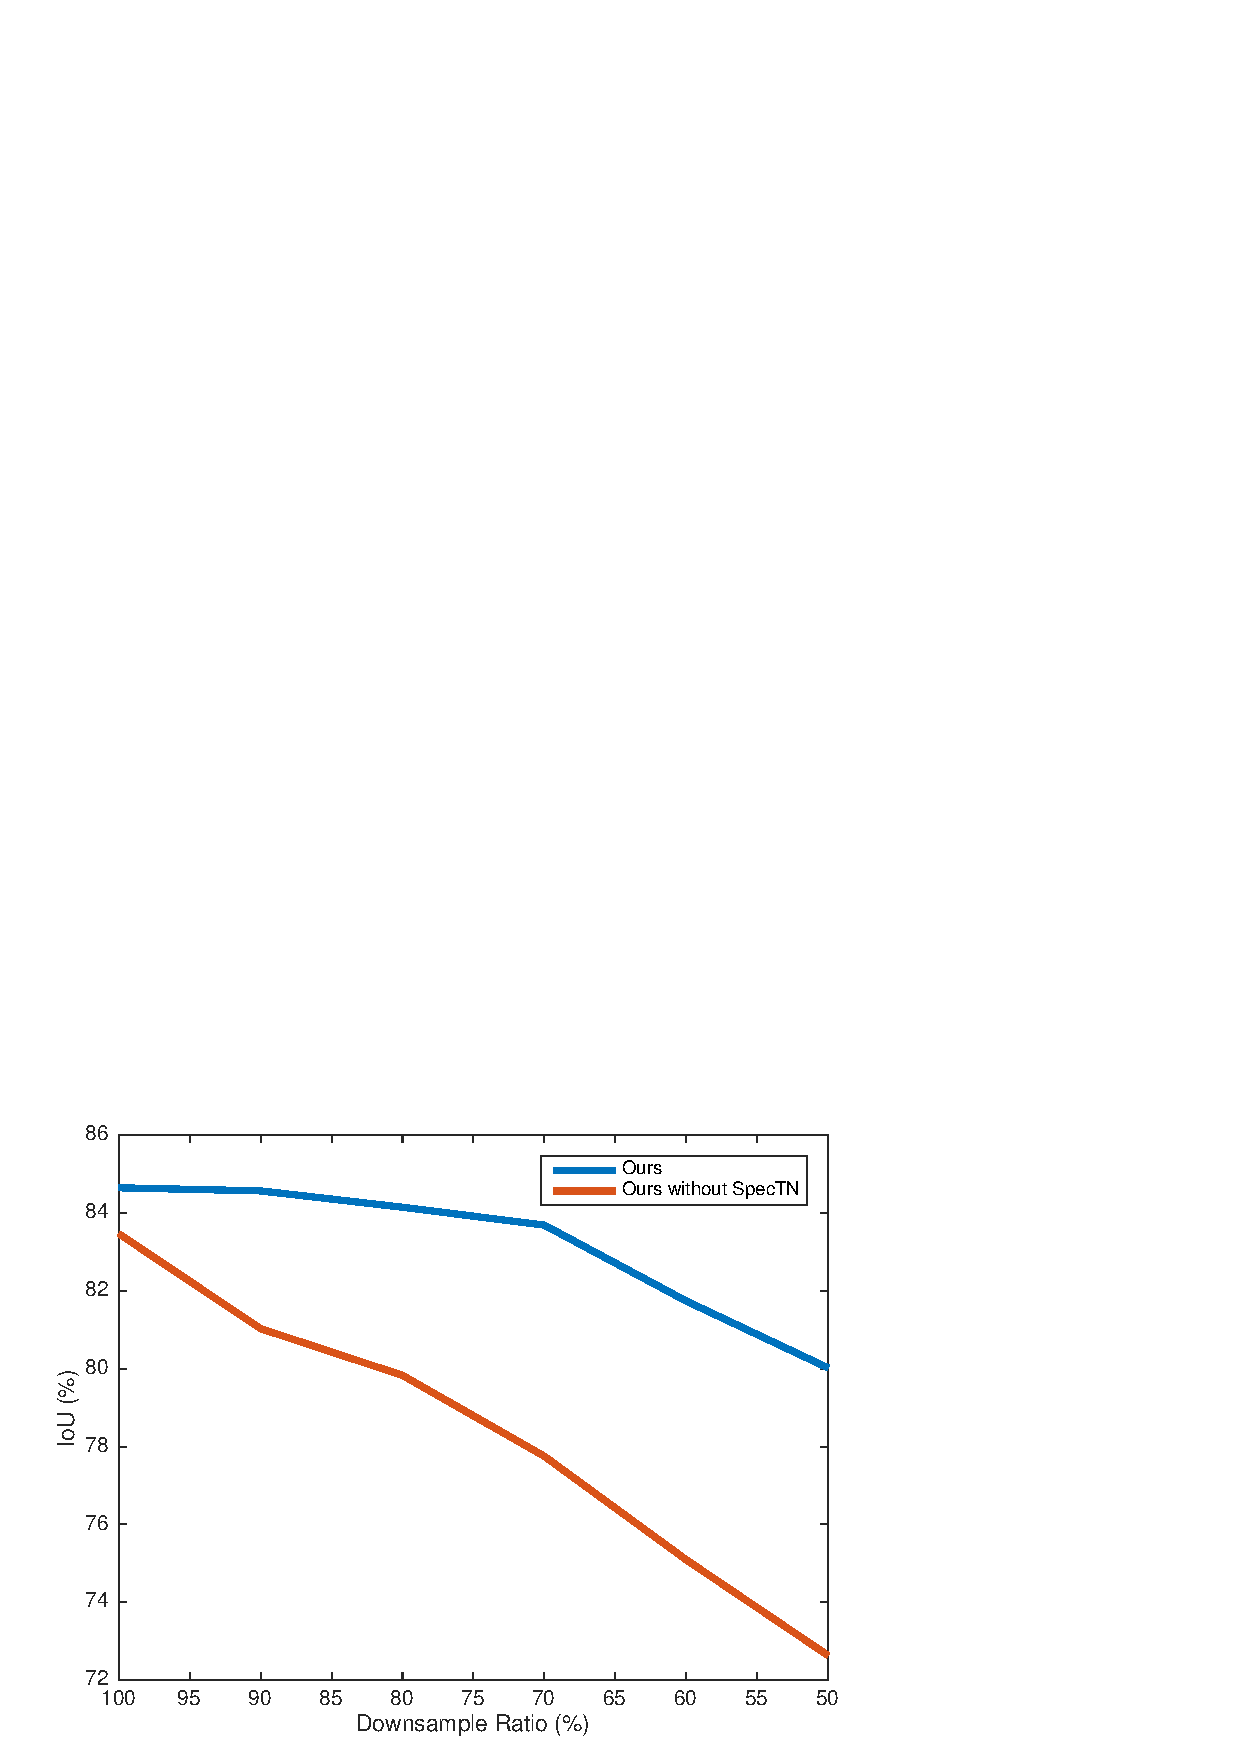
\includegraphics[width=0.8\linewidth]{./fig/downsample.pdf}
 \caption{We evaluate the robustness of our model to sampling density change. Test shapes are downsampled by different ratios and fed into our network. We compute the segmentation IoU for different downsample ratios and show it here. With SpecTN, our framework becomes more robust to sampling density change.}
 \label{fig:downsample}
\end{figure}

%\todo{Visualize joint basis}

\subsection{Qualitative Results and Error Analysis}
Figure~\ref{fig:erroranalysis} shows segmentation results generated from our network on two categories, Chair and Lamp. Representative good results are shown in the first block and  typical error patterns are summarized from the second to fourth blocks.

Most of our segmentation is very close to ground truth as is shown in the first block. We can accurately segment shapes with large geometric or topological variations like wide bench v.s. ordinary chair, pendant lamp v.s. table lamp. The lamp base on the first row and the lampshade on the second row are very similar regarding their local geometry; however, since our network is able to capture large scale context information, it could still differentiate the two and segment shapes correctly.

We observe several typical error patterns in our results. Most segmentation error occurs along part boundaries. %Our network sometimes generates fuzzy part boundaries, especially if the underlying part segments have a very smooth normal transition, as is shown in the second row of the second block. 
There are also cases where the semantic definition of parts has inherent ambiguities. %In these cases, our network may generate predictions slightly different from the ground truth but are still reasonable. 
We also observe a third type of error pattern, in which our prediction might miss a certain part completely, as is shown in the fourth block.

\begin{figure}
    \centering
    \includegraphics[width=\linewidth]{./fig/erroranalysis4.pdf}
    \caption{We visualize some segmentation results from our network prediction. The first block shows typical correct segmentations, notice the huge shape variation we can cover. The second to fourth blocks summarize different error patterns we observe in the results.}
    \label{fig:erroranalysis}
\end{figure}

\iffalse
\todo{
Compare different alternatives of our method
\begin{itemize}
    \item with multiple representatives instead of a single canonical space for spectral synchronization
    \item without join basis learning, visualize joint basis
    \item without dilated kernel, visualize dilated kernel
    \item different kernel choice: polynomial, cubic splines, exponential window, modulated exponential window
    \item different input vertex functions, extrinsic vertex functions help much since it's essentially a combination between extrinsic and intrinsic information for segmentation. intrinsic feature might not help much since the network is intrinsic and captures quite a lot intrinsic information already.
    \item network design, with/without skip link
\end{itemize}
}
\fi

\vs
\section{Conclusion}\label{sec:ccl}
\vsb
In this paper, we have proposed a new methodology for combining kernels
and convolutional neural networks. We show that  
mixing the ideas of these two concepts is fruitful,
since we achieve near state-of-the-art performance 
on several datasets such as MNIST, CIFAR-10, and STL10, with simple architectures
and no data augmentation.
Some challenges regarding our work are left open for the future. The first one
is the use of supervision to better approximate the kernel for the prediction
task. The second consists in leveraging the kernel interpretation of our
convolutional neural networks to better understand the theoretical properties
of the feature spaces that these networks produce.



\vsb
\subsubsection*{Acknowledgments}
\vsb
This work was partially supported by grants from ANR (project MACARON ANR-14-CE23-0003-01),
MSR-Inria joint centre, European Research Council (project ALLEGRO), CNRS-Mastodons program (project GARGANTUA), and the LabEx PERSYVAL-Lab (ANR-11-LABX-0025).

\newpage
\small{
   \bibliographystyle{plain}
   \bibliography{abbrev,main}
}
 \appendix
 \section{Positive Definiteness of~$K$}\label{sec:appendixA}
To show that the kernel~$K$ defined in~(\ref{eq:kernel}) is positive definite
(p.d.), we simply use elementary rules from the kernel literature described in
Sections 2.3.2 and 3.4.1 of~\cite{shawe2004}.  A linear combination of p.d. kernels with non-negative weights is also p.d. (see Proposition 3.22
of\cite{shawe2004}), and thus it is sufficient to show that for all $\z,\z'$
in~$\Omega$, the following kernel on $\Omega \to \HH$ is p.d.:
\begin{displaymath}
   (\varphi,\varphi') \mapsto \big\|\varphi(\z)\big\|_\HH  \normH{\varphi'(\z')} e^{-\frac{1}{2\sigma^2} \normH{\tildephi(\z)-\tildephi'(\z')}^2}.
\end{displaymath}
Specifically, it is also sufficient to
show that the following kernel on $\HH$ is p.d.:
\begin{displaymath}
   (\phi,\phi') \mapsto \big\|{\phi}\big\|_\HH  \normH{\phi'} e^{-\frac{1}{2\sigma^2} \normH{\frac{\phi}{\|\phi\|_\HH}-\frac{\phi'}{\|\phi'\|_\HH}}^2}.
\end{displaymath}
with the convention $\phi/\|\phi\|_\HH=0$ if~$\phi=0$.
This is a pointwise product of two kernels and is p.d. when each of the two
kernels is p.d. The first one is obviously p.d.: $(\phi,\phi') \mapsto
\|{\phi}\|_\HH  \normH{\phi'}$. The second one is a composition of the Gaussian
kernel---which is p.d.---, with feature maps $\phi/\|\phi\|_\HH$ of a
normalized linear kernel in~$\HH$.  This composition is p.d. according to
Proposition 3.22, item (v) of~\cite{shawe2004} since the normalization does
not remove the positive-definiteness property.

\section{List of Architectures Reported in the Experiments}\label{appendix:arch}
We present in details the architectures used in the paper in Table~\ref{table:arch}.
\begin{table}[hbtp]
   \centering
   \begin{tabular}{|*{9}{c|}}
      \hline
      Arch. & $N$ & $m_1$  & $p_1$  &  $\gamma_1$ & $m_2$ &  $p_2$ & $S$  &  $\sharp$ param\\
      \hline
      \hline
      \multicolumn{9}{|c|}{MNIST} \\
      \hline
      CKN-GM1 & 2 &  $1 \times 1$  &  12  & 2 &  $3 \times 3$ &  50 &  $4 \times 4$ & $5\,400$\\
      \hline
      CKN-GM2 & 2 &  $1 \times 1$  &  12  & 2 &  $3 \times 3$ &  400 &  $3 \times 3$& $43\,200$ \\
      \hline
      CKN-PM1 & 1 &  $5 \times 5$  &  200  & 2 &  - &  - &  $4 \times 4$  & $5\,000$ \\
      \hline
      CKN-PM2 & 2 &  $5 \times 5$  &  50  & 2 &  $2 \times 2$ &  200 &  $6 \times 6$ & $41\,250$ \\
      \hline
      \hline
      \multicolumn{9}{|c|}{CIFAR-10} \\
      \hline
      CKN-GM & 2 &  $1 \times 1$  &  12  & 2 &  $2 \times 2$ & 800 &  $4 \times 4$ & $38\,400$\\
      \hline
      CKN-PM & 2 &  $2 \times 2$  &  100  & 2 &  $2 \times 2$ &  800 &  $4 \times 4$ & $321\,200$\\
      \hline
      \hline
      \multicolumn{9}{|c|}{STL-10} \\
      \hline
      CKN-GM & 2 &  $1 \times 1$  &  12  & 2 &  $3 \times 3$ & 800 &  $4 \times 4$ & $86\,400$\\
      \hline
      CKN-PM & 2 &  $3 \times 3$  &  50  & 2 &  $3 \times 3$ &  800 &  $3 \times 3$ & $361\,350$\\
      \hline

   \end{tabular}
   \caption{List of architectures reported in the paper. $N$ is the number of layers; $p_1$ and~$p_2$ represent the number of filters are each layer; $m_1$ and~$m_2$ represent the size of the patches~$\NN_1$ and~$\NN_2$ that are of size~$m_1 \times m_1$ and~$m_2 \times m_2$ on their respective feature maps~$\zeta_1$ and~$\zeta_2$; $\gamma_1$ is the subsampling factor between layer 1 and layer 2; $S$ is the size of the output feature map, and the last column indicates the number of parameters that the network has to learn.}
   \label{table:arch}
\end{table}



\end{document}
